
\section{Einleitung}
Unter Beugung von Licht wird die Ablenkung von Licht an Hindernissen verstanden.
Dabei kommt es zur Abweichung von der geometrischen Optik.
Mithilfe des Huygenschen Prinzip lassen sich allerdings die Beugungsbilder erklären.
\newline
Dieser Versuch wird an zwei Einspalten und an einem Doppelspalt durchgeführt, wobei
zum Schluss das Beugungbild des Doppelpalts mit dem eines Einzelspalts verglichen wird.
\section{Theorie}
Zur Untersuchung von Lichtbeugung wird unter der Fresnelschen und der Fraunhoferschen
Beugung unterschieden.
\newline
Bei der Fresnelschen Beugung (Abbildung \ref{fig:1} a)) kommt es zur Interferenz
divergenter Strahlenbündel, die unter verschiedenen Winkel gebeugt wurden im Beobachtungspunkt P.
Dabei liegen die Lichtquelle und der Beobachtungspunkt im Endlichen.\newline
Bei der Fraunhoferschen Beugung hingegen liegt die Lichtquelle im Unendlichen. Dadurch
kommt es zur Beugung eines paralleln Lichtbündels mit einer eben Wellenfront. Mithilfe einer
Sammellinse kann das Strahlenbündel in die Brennebene abgebildet werden. Dies hat zur Konsequenz,
dass die Strahlen im Beobachtungspunkt interferieren und im selben Winkel gebeugt werden.
\newline
\begin{figure}
 \centering
  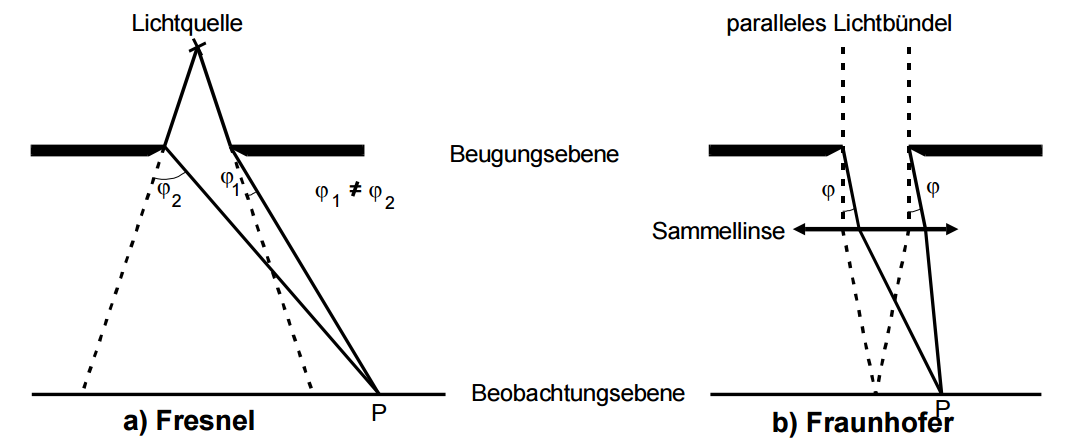
\includegraphics[scale=0.5]{bild1.png}
  \caption{Fresnelsche und Fraunhofersche Beugung im Vergleich.\cite{on1}}
  \label{fig:1}
\end{figure}
\newline
In diesem Versuch wird nur die Fraunhofersche Anordnung betrachtet. Die Fraunhofersche
Beugung bezieht sich auf das Huygensche Prinzip. Dieses besagt, dass von jedem Punkt einer
Welle eine Kugelwelle ausgeht. Durch die Interferenz dieser Elemtarwellen entsteht eine
neue Wellenfront.
\newline
Die Feldstärke einer aus z-Richtung einfallende Welle wird mit
\begin{equation}
  A(z,t) = A_0 \exp(\symup{i}(\omega t - 2\pi z/\lambda))
\end{equation}
berechnet. Die Phasendifferenz zwischen den einzelnen Strahlen ist
\begin{equation}
  \delta = \frac{2\pi s}{\lambda} = \frac{2\pi x \sin\varphi}{\lambda} \,,
\end{equation}
was in der folgenden Abbildung \ref{fig:2} deutlich wird.
\begin{figure}
  \centering
  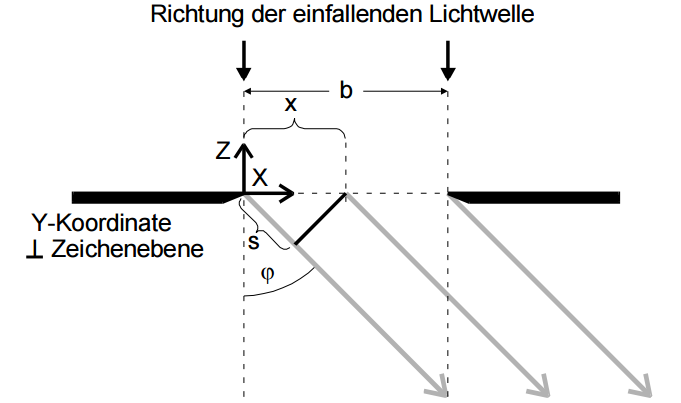
\includegraphics[scale=0.5]{bild2.png}
  \caption{Phasenbeziehung zweier Strahlen\cite{on1}}
  \label{fig:2}
\end{figure}

\newpage
Aufgrund der infinitismal kleinen Breite der Strahlen wird über die gesamte Spaltbreite b integriert.
Daraus ergibt sich für die Amplitude in $\varphi$-Richtung:
\begin{equation}
  B(z,t,\varphi) = A_0 \exp\left(\symup{i}\left(\omega t - \frac{2\pi z}{\lambda}\right)\right)
                        \exp\left(\frac{\pi \symup{i}b\sin\varphi}{\lambda}\right)
                  \frac{\lambda}{\pi \sin\varphi}\sin\left(\frac{\pi b \sin\varphi}{\lambda}\right) \,.
\end{equation}
Da sich die Amplituden wegen den sehr hohen Lichtfrequenzen nicht messbar sind, muss die gemittelte
Intensität betrachtet werden
\begin{equation}
  I(\varphi) \propto B(\varphi)^2 = A_0^2 b^2 \left(\frac{\lambda}{\pi b \sin\varphi}\right)^2 \sin^2\left(\frac{\pi b \sin\varphi}{\lambda}\right).
\label{eqn:reg}
\end{equation}

\begin{figure}
  \centering
  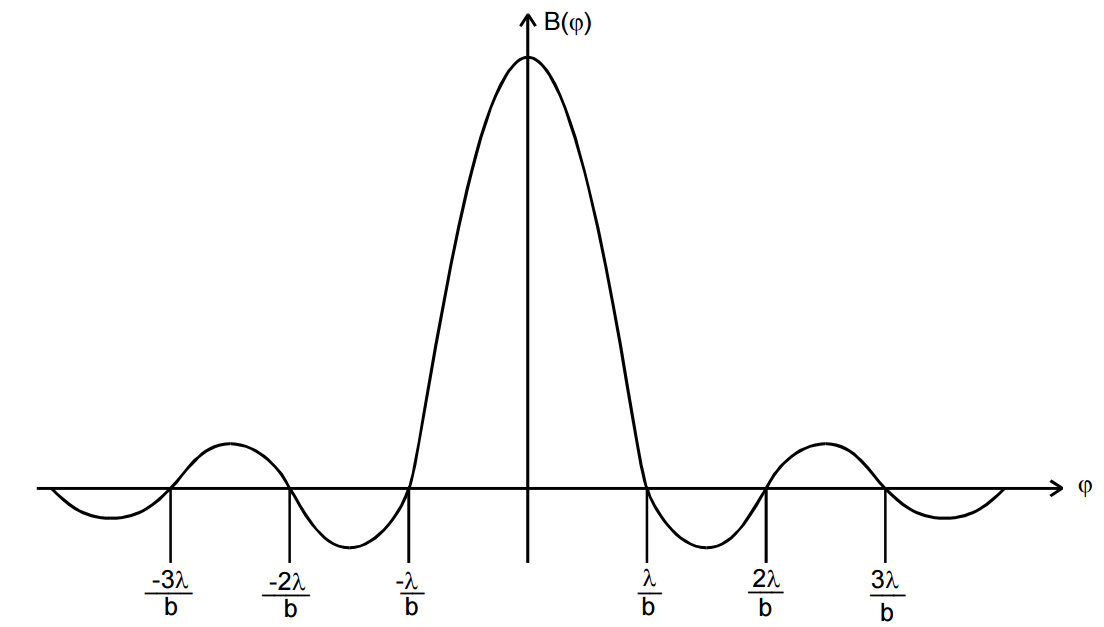
\includegraphics[scale=0.4]{bild3.png}
  \caption{Amplitudenverteilung an einem Parallelspalt\cite{on1}}
  \label{fig:3}
\end{figure}
\subsection{Beugung am Doppelspalt}
Bei einem Doppelspaltversuch wird die Intensitätsverteilung vom parallelen Licht durch
\begin{equation}
 I(\varphi) \propto B(\varphi)^2 = 4\cos^2\left(\frac{\pi s \sin\varphi}{\lambda}\right) \left(\frac{\lambda}{\pi b \sin\varphi}\right)^2
                                    \sin^2\left(\frac{\pi b \sin\varphi}{\lambda}\right) \,,
\label{eqn:aus}
\end{equation}
beschrieben. Dabei ist wie in Abbildung \ref{fig:4} zu sehen ist, die Beugungsverteilung des Doppelspalts
eine Überlagerung von zwei Einzelspalten mit der Breite b im Abstand s.

\begin{figure}
  \centering
  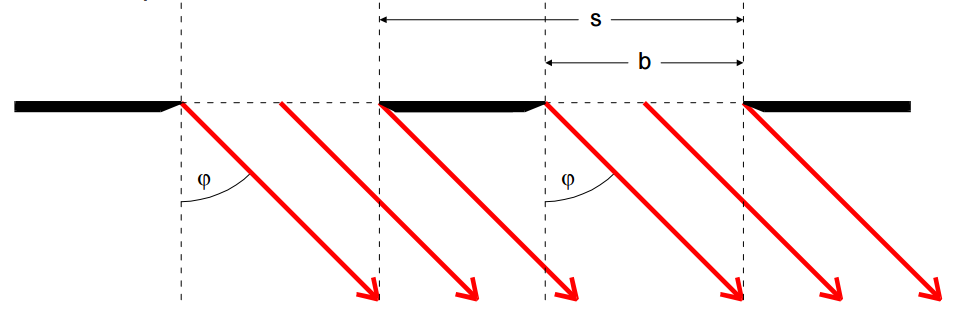
\includegraphics[scale=0.5]{bild4.png}
  \caption{Beugung am Doppelspalt\cite{on1}}
  \label{fig:4}
\end{figure}
\section{Durchführung}
Der Versuch wird wie in Abbildung \ref{fig:5} zu sehen ist, aufgebaut. In einer Entfernung
von mindestens einem Meter wird ein He-Ne-Laser als Lichtequelle zur Beleuchtung des
Photoelementes verwendet.
\begin{figure}
  \centering
  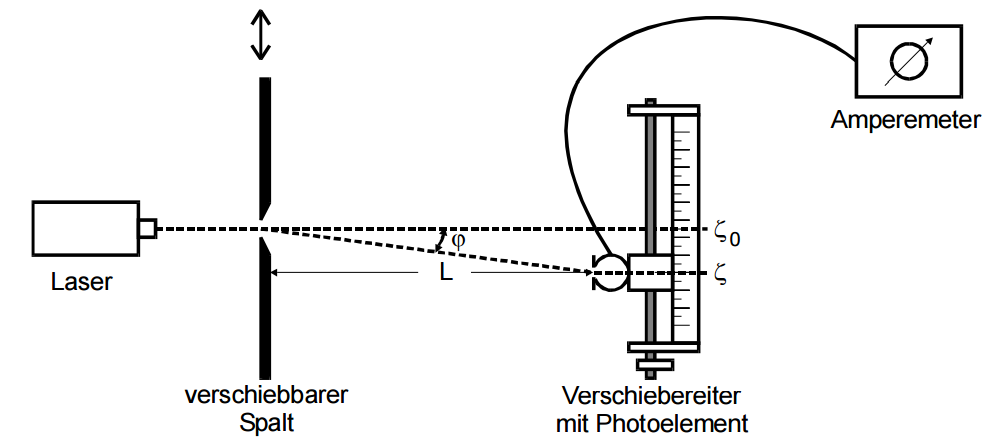
\includegraphics[scale=0.5]{aufbau.png}
  \caption{Versuchsaufbau\cite{on1}}
  \label{fig:5}
\end{figure}
\newline
Als erstes wird der Dunkelstrom der Photoelektrode gemessen. Dieser muss von jedem weiteren Messwert
abgezogen werden.\newline
Der Beugungswinkel $\varphi$ wird aus der Detektorstellung $\zeta$ bestimmt. Dabei ist
$\zeta_0$ die Detektorstellung des ungebeugten Strahls
\begin{equation}
  \varphi \approx \tan\varphi = \frac{\zeta - \zeta_0}{L}.
\end{equation}
